% !TeX root = ../main.tex
\section{Methods}\label{sec:methods}



We developed Windowed CUSUM to detect recurrent stand disturbances from near-decadal Sentinel-1 time series and reconstruct plantation turnover histories. The workflow comprised stand-level time-series construction, recurrent-event detection, spatially structured evaluation, and rotation-history reconstruction (Fig.~\ref{fig:workflow}).


\begin{figure}[pos=!htbp]
    \centering
    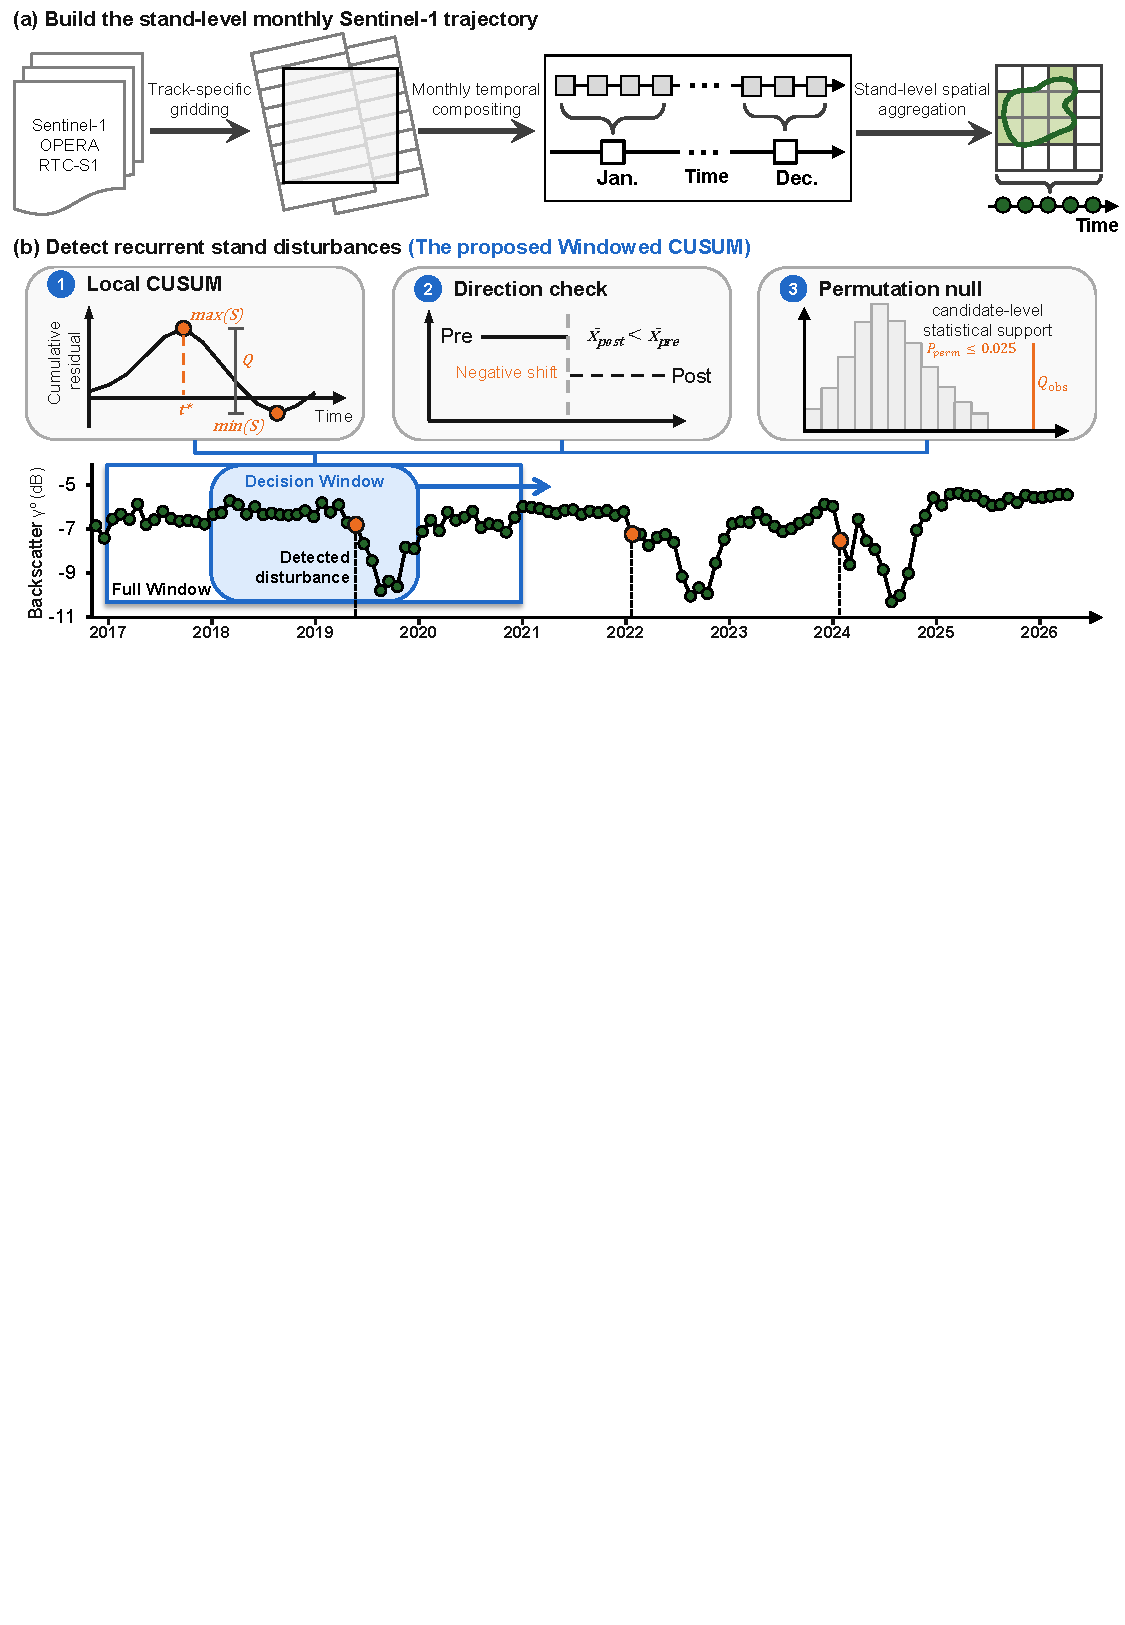
\includegraphics[width=0.85\linewidth]{figures/fig03_workflow.pdf}
    \caption{Overall methodological framework for recurrent stand-disturbance detection and plantation-rotation analysis.}
    \label{fig:workflow}
\end{figure}

\subsection{Sentinel-1 monthly time-series construction and stand representation}
\label{sec:s1_timeseries_representation}
Track-specific monthly series were constructed with S1-GRiTS (\url{https://github.com/ottoKae/S1-GRiTS}), retaining pass direction, relative orbit, and polarization. Let $\gamma_{\mathrm{dB},p,a,r}^{0,(q)}$ denote RTC backscatter for grid cell $p$, acquisition $a$, track $r$, and polarization $q\in\{\mathrm{VV},\mathrm{VH}\}$. Monthly backscatter was as shown in Equation~\eqref{eq:pixel_monthly_median}.
\begin{equation}
    \label{eq:pixel_monthly_median}
    y_{p,t,r}^{(q)}
    =
    \operatorname{median}
    \left\{
    \gamma_{\mathrm{dB},p,a,r}^{0,(q)}:
    a\in\mathcal{A}_{p,t,r}
    \right\},
\end{equation}
where $\mathcal{A}_{p,t,r}$ contains valid acquisitions in month $t$.
Missing months remained missing and were not interpolated.

For polygon $G_m$, the primary Polygon-first trajectory was the median of finite monthly values whose grid-cell centres fell within the polygon in Equation~\eqref{eq:polygon_monthly_median}. Grid cells contributed equally, and track-specific trajectories remained.
separate until event consolidation.
\begin{equation}
    \label{eq:polygon_monthly_median}
    x_{m,t,r}^{(q)}
    =
    \operatorname{median}
    \left\{
    y_{p,t,r}^{(q)}:
    \mathbf{c}_p\in G_m
    \right\}.
\end{equation}




Alternative spatial representations were evaluated to test the sensitivity of disturbance detection to stand representation. Polygon-first alternatives comprised the spatial mean, histogram mode, and nearest representative grid cell. Pixel-first alternatives retained individual grid-cell trajectories through disturbance detection and subsequently consolidated candidate evidence using eight-neighbour support, temporal DBSCAN, or joint space--time DBSCAN~\citep{Ester1996DBSCAN}. Parameters required by the Pixel-first strategies were selected exclusively from spatial training data as described in Section~\ref{sec:experimental_evaluation}.


\subsection{The proposed Windowed CUSUM}\label{sec:windowed_cusum}

The proposed Windowed CUSUM was designed to detect recurrent negative departures in stand-level Sentinel-1 backscatter using a sequence of overlapping local-reference windows. Each window establishes an updated local statistical context, allowing recurrent changes to be evaluated throughout the observation period without permanently segmenting the time series after each detected event. Figure~\ref{fig:windowed_cusum_concept} provides a visual overview of how overlapping local-reference windows, central-interval admission, the negative-shift constraint, and permutation screening jointly define an accepted candidate.

\begin{figure*}[pos=!htbp]
    \centering
    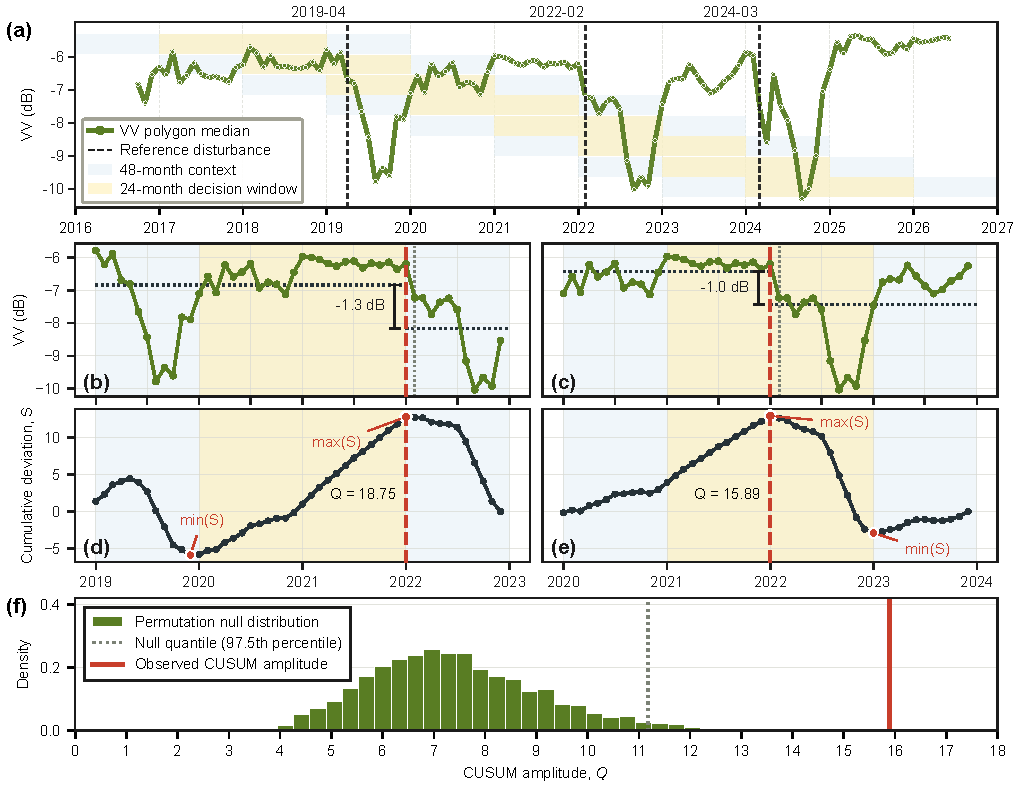
\includegraphics[width=\textwidth]{figures/fig04_windowed_cusum_concept.pdf}
    \caption{Conceptual illustration of Windowed CUSUM for one observed BALSA stand. (a) The stand-level VV trajectory with overlapping 48-month context windows, 24-month central decision windows, and dated disturbances. (b,c) Local-reference VV trajectories in two adjacent windows. (d,e) The corresponding cumulative-deviation curves: the candidate is rejected in (d) because it falls outside the central decision window, but retained in (e) because it falls within that window. (f) Evaluation of the retained CUSUM amplitude against its window-specific permutation null.}
    \label{fig:windowed_cusum_concept}
\end{figure*}


Windowed CUSUM was parameterized by the window length $W$ and the displacement $S$ between consecutive windows. For a window beginning at calendar month $b$, the full estimation window and central decision interval were defined as Equation~\eqref{eq:window_definition}. Each window required at least 12 finite observations; missing months were not interpolated, and boundary windows were clipped to the available record without temporal padding.
\begin{equation}
    \label{eq:window_definition}
    \mathcal{W}_b=[b,b+W),
    \qquad
    \mathcal{D}_b=[b+S,b+W-S),
\end{equation}
where $\mathcal{W}_b$ defines the temporal domain used to estimate the local CUSUM statistic, whereas $\mathcal{D}_b\subset\mathcal{W}_b$ defines the interval within which a candidate event can be admitted. The resulting decision-interval length is therefore $C=W-2S$. Thus, $W$ controls the local temporal context, while $S$ determines both the displacement between consecutive windows and the temporal margin excluded from candidate admission at each window boundary.


Within each local window, CUSUM was computed from the finite observations in temporal order. For notational simplicity, let $x_1,\ldots,x_n$ denote the finite observations extracted from the corresponding stand-level monthly trajectory, and let $\bar{x}$ denote their mean. The centred cumulative residual and CUSUM amplitude were defined in Equation~\eqref{eq:local_cusum}.
\begin{equation}
    S_t
    =
    \sum_{i=1}^{t}(x_i-\bar{x}),
    \qquad
    Q
    =
    \max_t S_t-\min_t S_t,
    \qquad
    t=1,\ldots,n .
    \label{eq:local_cusum}
\end{equation}
where $S_t$ is the cumulative residual at the $t$-th finite observation, $Q$ quantifies the magnitude of the strongest structural departure within the window, and $n$ is the number of finite observations. Thus, $S_t$ records the accumulated departure from the window mean as the trajectory is traversed chronologically, whereas $Q$ summarizes the overall strength of the resulting CUSUM signal.

For a persistent negative shift, positive deviations accumulate before the decline and negative deviations accumulate afterward. The cumulative residual therefore reaches a local maximum near the transition between the two states. The corresponding candidate change boundary was defined as~\citep{Page1954CUSUM,Ygorra2021CuSum} in Equation~\eqref{eq:candidate_position}.
\begin{equation}
    t^{*}
    =
    \arg\max_t S_t .
    \label{eq:candidate_position}
\end{equation}
Accordingly, $Q$ describes the magnitude of the local structural change, whereas $t^{*}$ identifies the candidate change location within the sequence of finite observations.



After mapping $t^*$ to calendar time, candidates outside $\mathcal{D}_b$ were discarded. Treating $x_{t^*}$ as the first post-change observation, we calculate in Equation~\eqref{eq:time_pre_post_mean}. A candidate was retained only when $\bar{x}_{\mathrm{post}}<\bar{x}_{\mathrm{pre}}$.
\begin{equation}
    \label{eq:time_pre_post_mean}
    \bar{x}_{\mathrm{pre}}
    =\operatorname{mean}(x_1,\ldots,x_{t^*-1}),
    \qquad
    \bar{x}_{\mathrm{post}}
    =\operatorname{mean}(x_{t^*},\ldots,x_n).
\end{equation}



Candidate support was evaluated against a window-specific permutation null rather than a common threshold on $Q$. Finite observations were randomly reordered and $Q$ recomputed for each permutation. The finite-sample-corrected $p$ value was in Equation~\eqref{eq:permutation_pvalue}~\citep{PhipsonSmyth2010Permutation}.
\begin{equation}
    p_{\mathrm{perm}}
    =
    \frac{
    1+\sum_{j=1}^{B}
    \mathbf{1}\{Q_j^{\mathrm{perm}}\ge Q_{\mathrm{obs}}\}
    }{B+1}.
    \label{eq:permutation_pvalue}
\end{equation}

The initial test used $B=3{,}999$; candidates with $0.015\le p_{\mathrm{perm}}\le0.035$ were recomputed with $B=19{,}999$. Candidates were retained at $p_{\mathrm{perm}}\le0.025$. This $p$ value refers only to the specified within-window null and is not a posterior disturbance probability or global false-discovery control.

Accepted candidates within one month were consolidated across overlapping windows and tracks. The representative month maximized track support, with the earliest month retained under ties.





\subsection{Experimental design and accuracy assessment}
\label{sec:experimental_evaluation}

\subsubsection{Reference-event protocol and spatial inference}


Historical signal characterization was separated from detector evaluation,
while spatial blocks were used to prevent information leakage and define
the unit of statistical resampling.

Absolute Sentinel-1 backscatter distributions were summarized from all valid polygon-month observations of the 3,498 validated BALSA polygons. Event-aligned analyses used the independently dated historical disturbance catalogue. For each polygon--track event, the pre-event background was defined as the median response from relative months $-12$ to $-3$ and required at least six finite observations. The paired event/post-event response was summarized over months 0 to $+2$ and required at least two finite observations. For the event-aligned trajectories, monthly responses were expressed relative to the same pre-event background and aligned by reference-event month. Track-specific responses were then fused by their median within each dated polygon event so that each event contributed once. These temporal-support criteria retained 1,018 events for the paired and event-aligned signature analyses, whereas all 1,093 reference-dated events from 462 polygons remained eligible for detector evaluation. Uncertainty in the paired and event-aligned signature summaries was estimated from 5,000 bootstrap resamples of complete spatial blocks.


The 1,093 reference events were grouped into 57 spatial blocks. All polygons, tracks, grid cells, and events from a block remained together. For analyses requiring parameter selection, the blocks were assigned to five event-balanced outer folds; parameters were selected on four folds and applied once to the held-out fold. The five held-out prediction sets were concatenated to obtain spatial out-of-fold estimates. Fixed-configuration analyses used the same blocks for paired inference without additional selection.



Detected and reference events were matched one-to-one within the prespecified $\pm2$-month tolerance, first maximizing the number of matches and then minimizing total absolute temporal lag. Precision, recall, and F1 were calculated at event level, and temporal mean absolute error (MAE) among matched pairs. Unmatched detections were not treated as independently verified false disturbances because the reference catalogue was not exhaustive.


The dated polygon event was therefore the unit of detector assessment, whereas the complete spatial block was the unit of statistical resampling. Paired 95\% confidence intervals for method and configuration contrasts were estimated from 5,000 bootstrap resamples of the 57 spatial blocks, using identical resamples for the quantities being compared~\citep{Davison1997Bootstrap}.


\subsubsection{Configuration sensitivity and component attribution}
\label{sec:configuration_component}

All configuration and component analyses followed the reference-event matching and spatial-inference protocol defined above. Whenever a representation or configuration required data-driven parameter selection, selection was restricted to the corresponding spatial training folds; analyses of locked configurations did not reopen parameter selection.

Sensitivity to stand representation was evaluated with the detector fixed at a 48-month window, 12-month displacement, and finite-sample permutation threshold of $p_{\mathrm{perm}}\leq0.025$. The Polygon-first median was compared with Polygon-first mean, histogram mode, and a representative-cell medoid, as well as Pixel-first connected support, temporal DBSCAN, and joint space--time DBSCAN~\citep{Ester1996DBSCAN}. Parameters required by the Pixel-first strategies were selected exclusively within the spatial training folds. Paired F1 contrasts were calculated relative to the Polygon-first median using the common spatial-block resampling protocol.

Window sensitivity evaluated $W\in\{24,36,48,60,72\}$ months and $S\in\{6,12\}$ months; 24/12 was excluded because its central decision interval was empty. A nested analysis selected geometry on the four training folds and evaluated it on the held-out fold. The previously locked 48/12 configuration remained unchanged for fixed operational analyses. Polarization sensitivity was evaluated under the retained Polygon-first representation and 48/12 geometry using VV-only, VH-only, either-polarization, and VV--VH agreement strategies.


Component attribution was evaluated only under the fixed operational configuration. The progressive analysis began with a single-pass Global CUSUM applied to the complete trajectory~\citep{Page1954CUSUM} and sequentially added local-reference windows, central-interval admission, the negative-shift constraint, and permutation-based screening. Only the complete configuration was designated the proposed Windowed CUSUM. A complementary controlled-removal analysis started from the complete detector and removed one component at a time while holding stand representation, missing-data treatment, candidate consolidation, track fusion, and event matching fixed. Adjacent progressive contrasts and full-minus-removed contrasts were evaluated using paired spatial-block resampling, with Holm adjustment applied to the four prespecified adjacent progressive comparisons. Reference polygons were additionally stratified by reference-event count to assess whether the effect of local-reference windowing was concentrated in recurrent-disturbance settings.


\subsubsection{Benchmark comparison and statistical robustness}
\label{sec:benchmark_robustness}

External benchmarking used the same reference catalogue, Polygon-first monthly trajectories, calendar support, event-matching rule, and spatial outer-fold structure defined above. Method-specific parameters were selected exclusively within the four spatial training folds before prediction on the held-out fold, and the five held-out prediction sets were concatenated for the final spatial out-of-fold comparison. Benchmark methods comprised maximum monthly decline, classical lower CUSUM~\citep{Page1954CUSUM}, ReCuSum~\citep{Ygorra2023ReCuSum}, a notebook implementation of factorized-polarization Bayesian online change-point detection~\citep{Bottani2026f-pol_BOCD}, and a BFAST-style seasonal one-break detector~\citep{Verbesselt2010BFAST}. Where decrease-filtered variants were evaluated, candidate events were additionally required to satisfy the same negative pre--post change direction used by Windowed CUSUM. Pairwise performance contrasts were quantified using the same paired spatial-block resampling scheme.

Temporal-null sensitivity changed only the permutation null while keeping the locked detector fixed. The finite-sample independent-value permutation~\citep{PhipsonSmyth2010Permutation} was compared with the previous empirical-rank implementation, 3-, 6-, and 12-month calendar-block permutations, residual moving-block-bootstrap nulls~\citep{Kunsch1989BlockBootstrap}, and a 3-month track-wise maximum-statistic null. All used an equivalent admission threshold of $p_{\mathrm{perm}}\le0.025$ and paired block inference. Monte Carlo stability was assessed across ten seeds for the stochastic null procedures. This analysis assessed robustness to temporal-null assumptions and did not reopen detector selection.








\subsubsection{Temporal truncation and prospective replay}
\label{sec:temporal_prospective}

Temporal truncation evaluated detection latency without changing the locked detector or the reference-event protocol defined above. For each historical reference event, the available Sentinel-1 record was truncated at $0$, $1$, $2$, $3$, $6$, and $12$ months after the reference month, and the fixed Windowed CUSUM configuration was replayed using only observations available up to the corresponding cutoff. No later observations were available to window construction, permutation screening, candidate consolidation, or track fusion. Recall and event-date stability were evaluated on a common-support cohort with sufficient temporal coverage at every horizon, allowing paired comparison without changes in the reference denominator. Uncertainty across truncation horizons was quantified using the same complete spatial blocks as the resampling units.

A separate prospective replay used observations available through June 2026 after all detector choices had been frozen. The 2026 manual review was excluded from representation, window, threshold, component, and benchmark selection. Candidate precision was estimated from a prespecified sample of detector-generated candidates, with the sampling fractions incorporated into the weighted estimates and spatial-block resampling used for uncertainty. Because review was conditioned on detected candidates rather than an independent sample of all disturbed and undisturbed polygons, the prospective analysis assessed candidate precision and operational behaviour but could not estimate missed disturbances or population recall.


\subsection{Stand-disturbance history reconstruction}
\label{sec:rotation_reconstruction}

The locked VV-only Windowed CUSUM was applied to each validated BALSA polygon to reconstruct its disturbance history during 2017--2025. For polygon $m$, the detected disturbance months were ordered as Equation~\eqref{eq:event_history} to form a temporally ordered event sequence,
\begin{equation}
    H_m^{(\mathrm{VV})}
    =
    (h_{m,1},h_{m,2},\ldots,h_{m,n_m}),
    \qquad
    h_{m,1}<h_{m,2}<\cdots<h_{m,n_m},
    \label{eq:event_history}
\end{equation}
where $h_{m,k}$ is the month of the $k$th detected disturbance and
$n_m$ is the observed stand-disturbance count. For spatial summaries,
$n_m$ was grouped as 0, 1, 2, and $\geq3$ detected disturbances.
The count refers only to disturbances observed within the Sentinel-1
record and therefore does not represent the absolute number of
plantation rotations.

Observed inter-disturbance intervals were calculated only between
consecutive detected disturbances in Equation~\eqref{eq:rotation_interval}.
\begin{equation}
    R_{m,k}^{\mathrm{obs}}
    =
    h_{m,k+1}-h_{m,k},
    \qquad
    k=1,\ldots,n_m-1,
    \label{eq:rotation_interval}
\end{equation}
where $R_{m,k}^{\mathrm{obs}}$ is the interval in months between adjacent
disturbance events. The first measurable interval therefore begins at
the first observed disturbance rather than the unknown planting date,
and intermediate events were never skipped to connect non-adjacent
disturbances. Uncertainty in interval summaries was estimated by
complete spatial-block bootstrap resampling.

Polarization robustness was assessed using a VH-supported subset of the
VV-defined intervals. An interval was classified as cross-polarization
consistent only when both bounding VV events had one-to-one VH matches
within $\pm2$ months. The original VV sequence was left unchanged:
unmatched intermediate VV events were retained and VH-only events were
not inserted. This subset was used only to assess polarization
sensitivity of the inter-disturbance interval distribution, not to
derive a separate VH-based rotation estimate.







